\documentclass{ximera}
%% handout
%% nohints
%% space
%% newpage
%% numbers


\prerequisites{none}

\title{Dependent and Independent Events}

\begin{document}
\begin{abstract}
We introduce the basic concept of probability and work through some simple examples.
\end{abstract}
\maketitle

\subsection*{Basic learning objectives}

These are the tasks you should be able to perform with reasonable fluency \textbf{when you arrive at our next class meeting}. Important new vocabulary words are indicated \emph{in italics}. 

\begin{itemize}
	\item Understand the distinction between \emph{dependent} and \emph{independent} events and perform calculations of each type.
    \item Understand \emph{the gambler's fallacy}.
\end{itemize}

\subsection*{Advanced learning objectives}

In addition to mastering the basic objectives, here are the tasks you should be able to perform \textbf{after class, with practice}: 

\begin{itemize}
	\item Understand the \emph{birthday paradox} and its associated calculations.
    \item Understand the importance of precise language and specifying conditions in advance when discussing probabilities as they pertain to \emph{coincidences}.
\end{itemize}

When talking about probability, two events are \emph{independent} if the outcome of one event does not influence the outcome of the other event. For example, if you were to flip a coin and roll a die, you would not expect that the outcome of the coin flip will change the probabilities on the die roll. This would make the events independent.

Two events are \emph{dependent} if the outcome of one event does have an influence on the outcome of the other event. Imagine you have an urn containing 2 red balls and 2 black balls, and you are planning to draw two balls from the urn (one at a time). The probability of getting a red ball on your second draw depends on what happened during your first draw. If you drew a black ball first, then there would be two red balls and one black ball in the urn, so that $P(\text{2nd draw red}) = \frac{2}{3}$. But if you had drawn a red ball the first time, then there would be one red ball and two black balls in the urn, and $P(\text{2nd draw red}) = \frac{1}{3}$. Since the first event influences the probability of the second event, these events are dependent.

An easy way to determine whether two events are dependent or independent is to look at the probability tree. If all of the branching at the second level is identical (including the probabilities), then the events are independent. If there is any difference in any of the branches, then the events are dependent.

For example, the following is the probability tree for drawing a ball from an urn containing two red balls, one white ball, and one blue ball, followed by flipping a biased coin.

\begin{image}
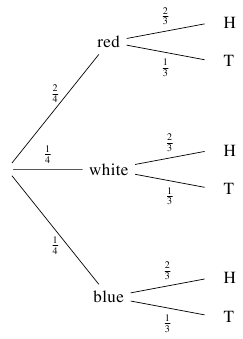
\includegraphics{ProbTree1.png}
%\begin{tikzpicture}[grow=right,level 1.style={level distance=2cm, sibling distance=2.5cm},level 2.style={level distance=2cm, sibling distance=.75cm}]
%\node{}
%    child {
%    	node[] {blue}
%        	child {
%            	node[label=right:{T}] {}
%                edge from parent
%                node[below] {\footnotesize $\frac{1}{3}$}
%            }
%            child {
%            	node[label=right:{H}] {}
%                edge from parent
%                node[above] {\footnotesize $\frac{2}{3}$}
%            }
%        edge from parent
%        node[below] {\footnotesize $\frac{1}{4}$}
%    }
%    child {
%    	node[] {white}
%        	child {
%            	node[label=right:{T}] {}
%                edge from parent
%                node[below] {\footnotesize $\frac{1}{3}$}
%            }
%            child {
%            	node[label=right:{H}] {}
%                edge from parent
%                node[above] {\footnotesize $\frac{2}{3}$}
%            }
%        edge from parent
%        node[above] {\footnotesize $\frac{1}{4}$}
%    }
%    child {
%    	node[] {red}
%        	child {
%            	node[label=right:{T}] {}
%                edge from parent
%                node[below] {\footnotesize $\frac{1}{3}$}
%            }
%            child {
%            	node[label=right:{H}] {}
%                edge from parent
%                node[above] {\footnotesize $\frac{2}{3}$}
%            }
%        edge from parent
%        node[above] {\footnotesize $\frac{2}{4}$}
%    };
%\end{tikzpicture}
\end{image}


If you focus on the part to the right of the red, white, and blue, you can see that they are completely identical. This means that drawing the ball and flipping the coin are independent.

The following is an example of a probability tree for drawing two balls without replacement from an urn containing 3 white balls and 5 black balls.

\begin{image}
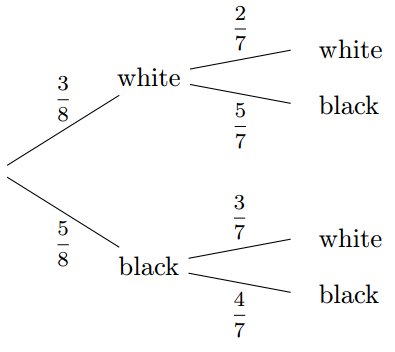
\includegraphics{ProbTree2.png}
%\begin{tikzpicture}[grow=right]
%\tikzstyle{level 1}=[level distance=2cm, sibling distance=2.5cm]
%\tikzstyle{level 2}=[level distance=2cm, sibling distance=.75cm]
%\node{}
%    child {
%    	node[] {black}
%        	child {
%            	node[label=right:{black}] {}
%                edge from parent
%                node[below] {\footnotesize $\frac{4}{7}$}
%            }
%            child {
%            	node[label=right:{white}] {}
%                edge from parent
%                node[above] {\footnotesize $\frac{3}{7}$}
%            }
%        edge from parent
%        node[below] {\footnotesize $\frac{5}{8}$}
%    }
%    child {
%    	node[] {white}
%        	child {
%            	node[label=right:{black}] {}
%                edge from parent
%                node[below] {\footnotesize $\frac{5}{7}$}
%            }
%            child {
%            	node[label=right:{white}] {}
%                edge from parent
%                node[above] {\footnotesize $\frac{2}{7}$}
%            }
%        edge from parent
%        node[above] {\footnotesize $\frac{3}{8}$}
%    };
%  \end{tikzpicture}
\end{image}

Even though the outcomes are the same, the probabilities of each outcome changes depending on which color was drawn first.

\begin{question}
Classify the following events as dependent or independent.
    \begin{hint}
    Dependent events are when the outcome of one event has an influence on the outcome of the other event. Independent events are when the outcome of one event does not influence the outcome of the other event.
    \end{hint}
    \begin{hint}
    Imagine that you're performing the experiment and think about what happens after the first event. Is this connected to what is about to happen in the next part?
    \end{hint}

\begin{itemize}
\item Removing two balls from an urn one at a time without replacement
\end{itemize}
\begin{multipleChoice}
      \choice{Independent}
      \choice[correct]{Dependent}
\end{multipleChoice}

\begin{itemize}
\item Removing two balls from an urn one at a time, but replacing the ball after each draw
\end{itemize}
\begin{multipleChoice}
      \choice[correct]{Independent}
      \choice{Dependent}
\end{multipleChoice}

\begin{itemize}
\item Flipping the same coin twice
\end{itemize}
\begin{multipleChoice}
      \choice[correct]{Independent}
      \choice{Dependent}
\end{multipleChoice}

\begin{itemize}
\item Flipping two different coins
\end{itemize}
\begin{multipleChoice}
      \choice[correct]{Independent}
      \choice{Dependent}
\end{multipleChoice}

\begin{itemize}
\item Dealing two cards from a standard deck of cards
\end{itemize}
\begin{multipleChoice}
      \choice{Independent}
      \choice[correct]{Dependent}
\end{multipleChoice}

\begin{itemize}
\item Dealing two cards from a deck of cards that contains no aces
\end{itemize}
\begin{multipleChoice}
      \choice{Independent}
      \choice[correct]{Dependent}
\end{multipleChoice}

\end{question}

The human mind is wired in a way that makes it good at spotting patterns. However, the idea of randomness is that there are no patterns. There is a desire to see patterns in randomness and to believe that independent events are actually dependent events. If you flip a fair coin and get heads 5 times in a row, you might think that you're due for a tail or that head is on a hot streak. Neither of these effects are real if the coin is fair. (If the coin is rigged in some way, all bets are off.)

This effect is known as the Gambler's Fallacy, and this concept extends beyond mathematics into cognitive psychology. The following video explains this concept in more detail: \youtube{https://www.youtube.com/watch?v=p14icOB2iac}



\begin{question}
The Gambler's Fallacy is the belief that...

    \begin{hint}
    The answer is in the video. The wording is slightly different, but the concept is the same.
    \end{hint}
    \begin{multipleChoice}
      \choice{--- you can beat the house when you gamble.}
      \choice[correct]{--- the chances of future events change based on previous events}
      \choice{--- superstitious acts can influence future outcomes}
      \end{multipleChoice}

\end{question}

\begin{question}
Which of the following are examples of the Gambler's Fallacy?
    \begin{hint}
    There are only four aces in a deck, so once all four are accounted for, there aren't any aces left.
    \end{hint}
    \begin{hint}
    If you keep flipping a coin it will eventually land heads.
    \end{hint}
    \begin{multipleChoice}
      \choice{If I keep flipping this quarter, eventually it will land heads.}
      \choice{Four aces have been dealt from this deck of cards. There's no way the next card will be an ace!}
      \choice[correct]{Our first child is going to be a girl because my mom's first child was a girl and my grandma's first child was a girl.}
      \end{multipleChoice}

\end{question}

\end{document}
